\chapter{Introdução}

\section{Arquitetura}
\begin{figure}
	\centering
		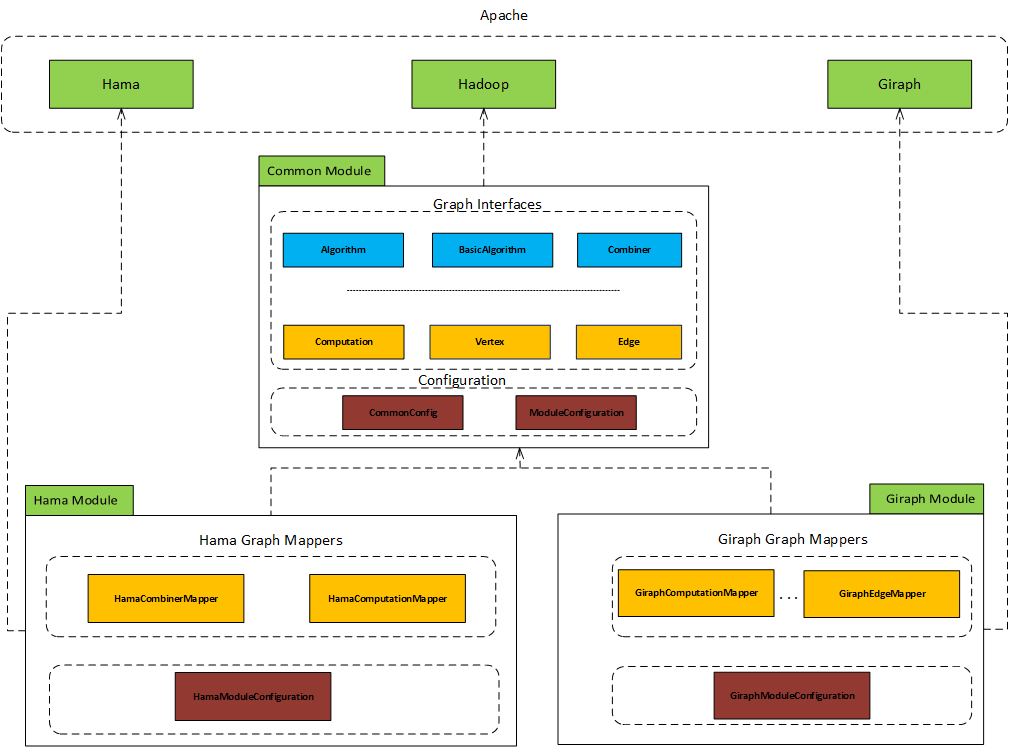
\includegraphics[width=\linewidth]{arquitetura}
	\caption{Em azul estão as interfaces e classes que devem ser implementadas por um programador que esteja interessado em implementar um algoritmo no módulo comum. As outras cores representam interfaces e classes que devem ser implementadas para criar-se um novo módulo sobre o módulo comum.}
	\label{fig:arquitetura}
\end{figure}


\section{Contextualização}
Nos últimos anos, o processamento de grandes quantidades de dados tem sido um tópico de grande interesse. Contudo, a análise das estruturas envolvidas no processo 
é normalmente complexa. De modo a diminuir a complexidade envolvida no tratamento deste tipo de estruturas surgiram algumas plataformas seguindo o modelo \textit{Map Reduce}, como o Apache Hadoop\cite{hadoop}.

O Apache Hadoop\cite{hadoop} é uma plataforma que visa facilitar o processamento e análise de estruturas de dimensões consideráveis em ambientes distribuídos, a qual tem sido muito utilizada.

A plataforma oferece um conjunto de benefícios tais como a sua interface simples de programação, escalabilidade e de ser tolerante a falhas.
Esta plataforma é composta por quatro módulos:
Hadoop Common (conjunto de ferramentas que servem de suporte a outros módulos),
Hadoop Distributed File System (sistema de ficheiros distribuído),
Hadoop Yarn (plataforma que disponibiliza o agendamento de tarefas)
e o Hadoop Map Reduce (módulo que usa o modelo de programação Map Reduce para o processamento de dados e agenda tarefas usando o Hadoop Yarn)

Apesar dos benefícios de se usar este tipo de plataforma para alguns tipos de dados, e ser possível a sua utilização para o processamento de redes através múltiplas invocações de Map Reduce, o modelo de programação usado  não é o mais adequado para o processamento de grafos devido à existência de  uma elevada complexidade envolvida na implementação de algoritmos e um custo computacional indesejado.
Para resolver este problema foi proposto pela Google uma plataforma, denominada Pregel\cite{pregel}, que se baseia no modelo de programação Bulk Synchronous Parallel\cite{bsp}.

Baseando-se na implementação da Google foram surgindo implementações \textit{open-source} como o GPS\cite{docgps}, Apache Hama\cite{hama} e Apache Giraph\cite{giraph}.
Estas plataformas exportam uma interface programável com algumas semelhanças assim como uma típica computação de um grafo, em que consiste começar por iniciar o respectivo grafo seguido de um número variável de \textit{supersteps} (iterações) até que todos os vértices estejam inactivos (não têm que participar na computação).
Durante cada \textit{superstep} é chamada (paralelamente) para cada vértice do grafo uma função definida pelo utilizador que irá delinear o seu comportamento.
Durante o processamento de um vértice, tem-se acesso às mensagem que lhe foram enviadas no \textit{superstep} anterior, sendo também possível enviar mensagens (que irão ser recebidas do próximo \textit{superstep}) para outros vértices que se conheça o seu identificador único (tipicamente vértices vizinhos).
Este modelo tem uma barreira de sincronização entre \textit{supersteps}, que faz com que cada um só se inicie após todos os \textit{nodes} entrarem na barreira de sincronização, fazendo com que a performance global seja afectada pelo \textit{node} que demore mais a processar.
De qualquer modo, o modelo simplifica a semântica da implementação dos algoritmos e tem normalmente um melhor desempenho que as implementações em Map Reduce devido à facilidade em que há em partilhar o estado entre os vários vértices. 


\section{Descrição do projecto}
Apesar de existirem alguns algoritmos implementados nos ambientes descritos anteriormente, o objectivo deste projecto é analisar as plataformas
baseadas no modelo \textit{Bulk Synchronous Parallel}, de modo a criar uma biblioteca modular que contenha um conjunto de algoritmos e que consiga
ser usada em diversas plataformas. As principais plataformas que serão estudadas para o desenvolvimento desta biblioteca será o Apache Hama e o Apache Giraph. 
O Apache Giraph é uma plataforma de interesse tendo em conta que usa como base o Apache Hadoop para o agendamento de tarefas, o que facilita o seu uso
para todas as infraestruturas que usam Apache Hadoop. O Apache Hama proporciona um modelo mais perto do \textit{Bulk Synchronous Parallel} que o Apache Giraph, daí também ser
alvo de estudo para esta biblioteca.


\section{Recursos}
Este projecto será desenvolvido com recurso a ferramentas e plataformas \textit{open source}.
As plataforma e ferramentas serão:
\begin{itemize}
 \item Java SDK 7
 \item Apache Hadoop
 \item Apache Giraph
 \item Apache Hama
\end{itemize}

O equipamento físico para obtenção de resultados sobre os algoritmos desenvolvidos será disponibilizado pelo INESC-ID. 
O equipamento inclui 8 maquinas virtuais com 1 CPU a 2.3GHz e 3GB de RAM tendo cada imagem 8Gb( havendo acesso a um disco extra de 32Gb) e o seu sistema operativo é Slackware 14.1 64bits.
As máquinas virtuais estão hospedadas em dois servidores dedicados cada um deles com 16Gb de RAM e 4 CPUs, em ambiente linux através de KVM.
